\documentclass[UTF8]{beamer}

\usetheme{Boadilla}
\usecolortheme{beaver}
\usefonttheme[onlymath]{serif}

\begin{document}

\title{FROG}
\subtitle{A Fast and Reliable Crowdsourcing Framework}
\author{ }
\institute{ }
\date{ }

\beamertemplatenavigationsymbolsempty

\frame{\titlepage}

\frame{\tableofcontents}

\AtBeginSection[]
{
    \begin{frame}
        \frametitle{Outline}
        \tableofcontents[currentsection]
    \end{frame}
}

\section{Introduction}

\subsection{Background}
\begin{frame}
    \frametitle{Crowdsourcing}
    
    \begin{block}{Definition of Crowdsourcing}
        Crowdsourcing is a sourcing model in which 
        individuals or organizations obtain goods 
        and services, including ideas and finances, 
        from a large, relatively open and often 
        rapidly-evolving group of internet users; 
        it divides work between participants to 
        achieve a cumulative result.
    \end{block}

    \begin{block}{Problems in Crowdsourcing Systems}
        \begin{itemize}
            \item Accuracy Problem
            \item Latency Problem
            \item (May) Lack of active workers
        \end{itemize}
    \end{block}
\end{frame}

\begin{frame}
    \frametitle{Accuracy and Latency Problems}
    \begin{figure}
        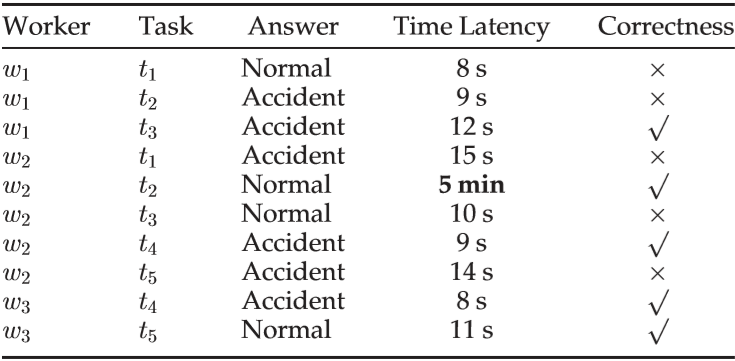
\includegraphics[width= 0.8\linewidth]{ACEXP.png}
        \label{fig:ACEXP}
        \caption{Example of Accuracy and Latency Problems in the Crowdsourcing System}
     \end{figure}
     \begin{center}
         High Latency: worker $w_2$ tags $t_2$ with \textbf{5 minutes}\\
         Low Accuracy: worker $w_2$ tags all pictures with 3 wrong labels
     \end{center}
\end{frame}

\begin{frame}
    \frametitle{The Problems}
    \begin{itemize}
        \item minimize the maximal latencies for all tasks
        \item maximize the accuracies (quality) of task results
        \item invite more offline workers to perform online tasks 
        when the system lacks of active workers
    \end{itemize}
\end{frame}

\begin{frame}
    \frametitle{Existing Studies}
    \begin{itemize}
        \item \textbf{[Rosenblatt 1956] and [Verroios 2015]}\ increases 
        prices over time to encourage workers to accept tasks
        to reduce the latency for \textbf{specific tasks}
        \item \textbf{iCrowd and CLAMShell}\ removes 
        low-accuracy or high-latency workers, which may lead 
        to \textbf{idleness of workers} and \textbf{low throughput of the 
        system}
    \end{itemize}
\end{frame}

\subsection{The FROG Framework}
\begin{frame}
    \frametitle{The FROG Approach}
    Two important components: 
    \textit{task scheduler} and \textit{notification module}
    \begin{block}{The Task Scheduler}
        \begin{itemize}
            \item actively schedules tasks for workers using
            heuristic algorithms
            \item considering both accuracy and latency
        \end{itemize}
    \end{block}
    
    \begin{block}{The Notification Module}
        \begin{itemize}
            \item notify offiine workers via invitation messages
            \item propose a \textit{smooth kernel density model} to 
            estimate the probabilities that workers 
            can accept task invitations
        \end{itemize}
    \end{block}
\end{frame}

\begin{frame}
    \frametitle{Illustration of the FROG framework}
    \begin{figure}
        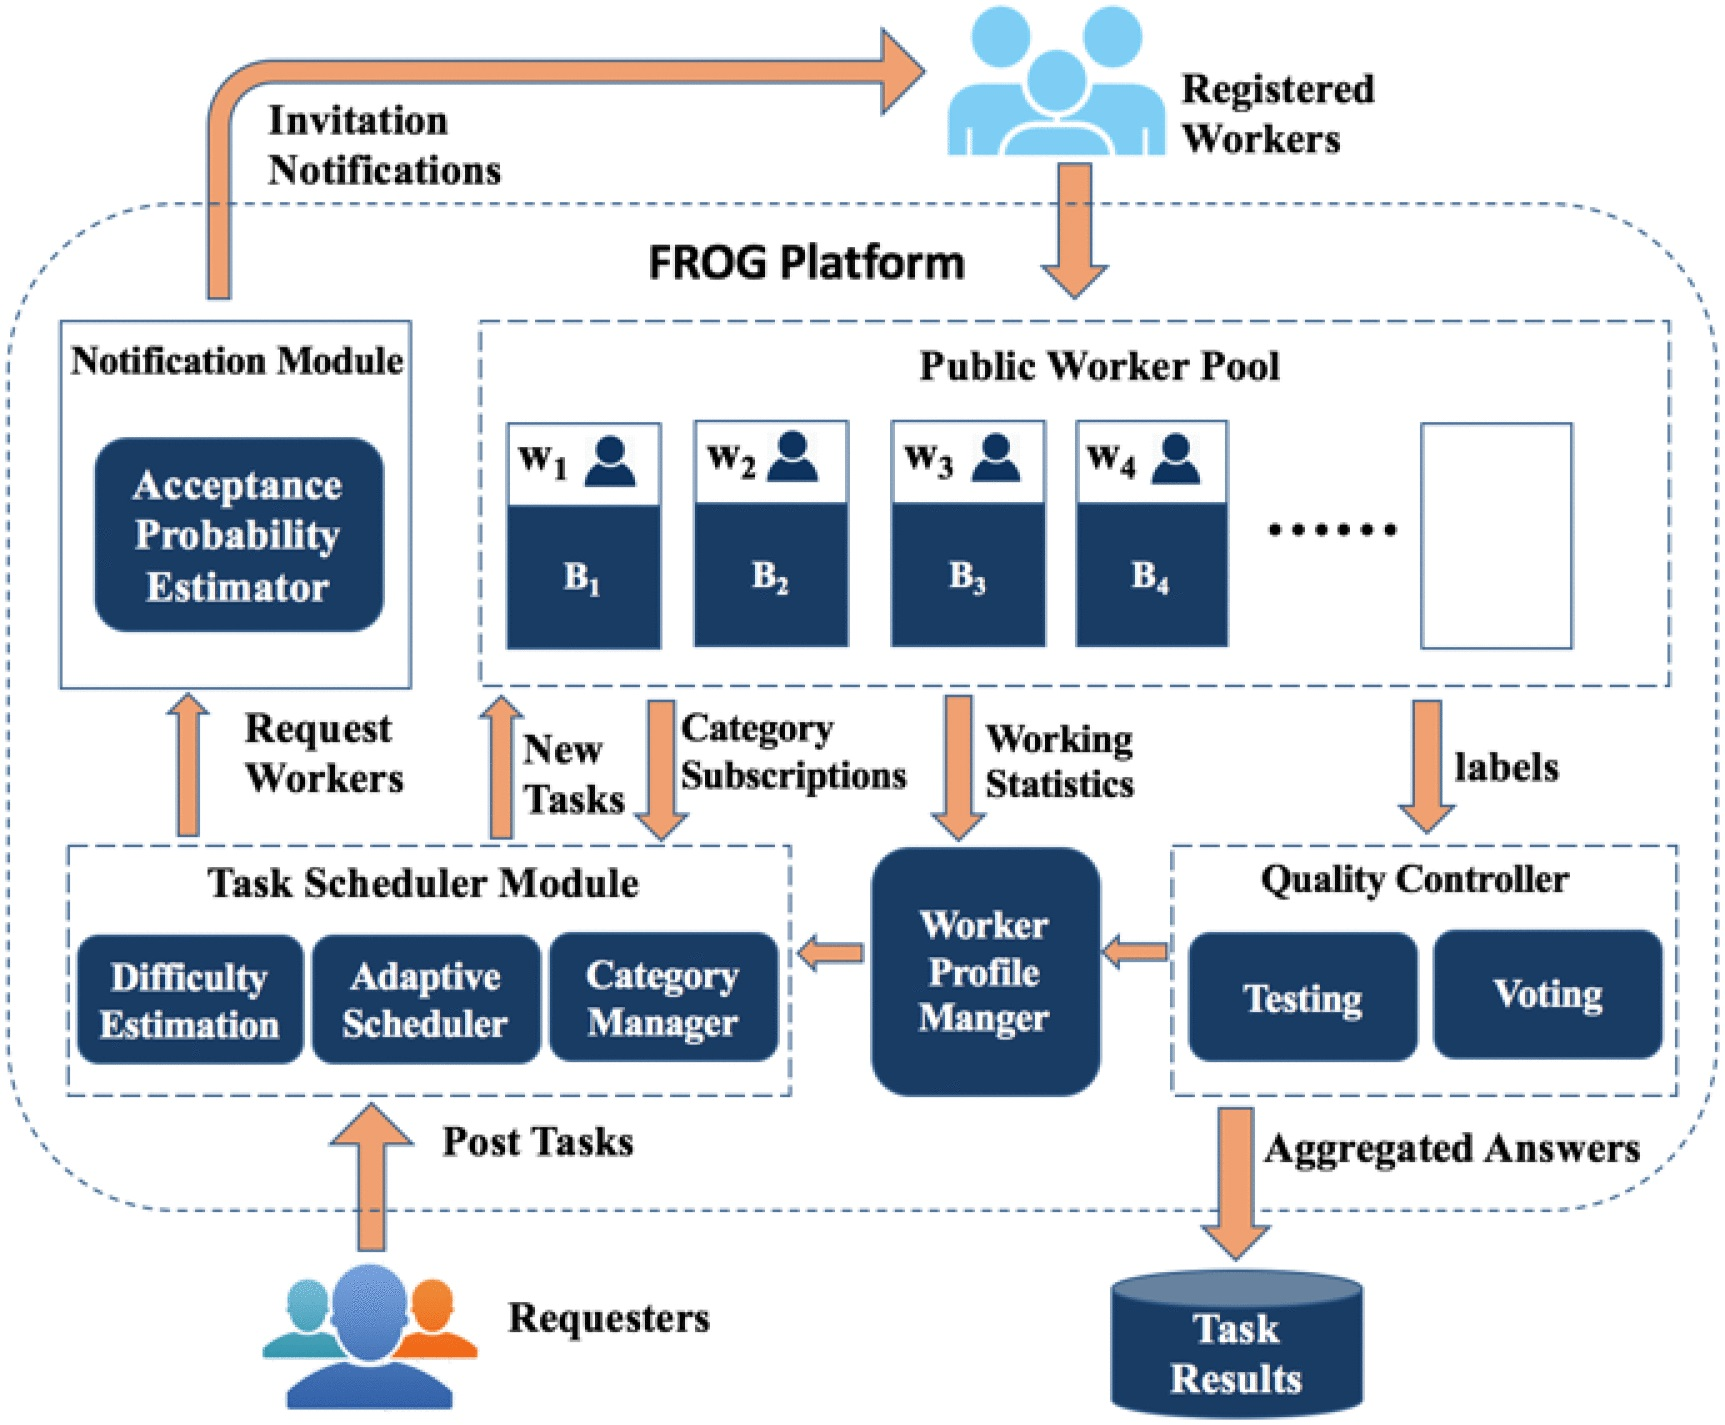
\includegraphics[width= 0.75\linewidth]{ILL.jpg}
     \end{figure}
\end{frame}

\begin{frame}
    \frametitle{Symbols and Descriptions}
    \begin{center}
        \begin{tabular}{ll}
        \hline
        Symbol & Description \\
        \hline
        $C$ &  a set of task categories $c_i$ \\  
        $T$ &  a set of tasks $t_i$  \\
        $W$ &  a set of workers $w_j$ \\
        $t_i.c$ &  the category of task $t_i$ \\
        $q_i$ &  a specific quality value of task $t_i$ \\
        $s_i$ &  the start time of task $t_i$ \\
        $f_i$ &  the finish time of task $t_i$ \\
        $a_{jl}$ & the category accuracy of worker $w_j$ on tasks in category $c_l$ \\
        $r_{jl}$ & the response time of worker $w_j$ on tasks in category $c_l$\\
        \hline
        \end{tabular}
        \end{center}
\end{frame}

\section{The Task Scheduler Module}
\subsection{Definitions}

\begin{frame}
    \frametitle{Tasks}
    \begin{itemize}
        \item $T = \{t1, t2, \cdots, t_m \}$ is a set of $m$ tasks in the crowdsourcing platform
        \item Each task $t_i$ belongs to a task category, $ti.c \in C$
        \item Each task $t_i$ arrives at the system at $s_i$
        \item Each task $t_i$ is associated with a user-specified quality 
        threshold $q_i$, which is the expected probability that the final
        result for task $t_i$ is correct
    \end{itemize}
\end{frame}

\begin{frame}
    \frametitle{Workers}
    \begin{itemize}
        \item $W = \{w_1, w_2, \cdots , w_n\}$ is a set of $n$ workers
        \item For tasks in category $c_l$, each worker $w_j$ 
        is associated with an accuracy, $a_{jl}$, that $w_j$ 
        do tasks in category $c_l$, and a response time, $r_{jl}$
    \end{itemize}
\end{frame}

\begin{frame}
    \frametitle{Expected Accuracy}
    The expected accuracy of task $t_i$ is:
    $$\operatorname{Pr}\left(W_{i}, c_{l}\right)=\sum_{x=\left\lceil\frac{k}{2}\right\rceil}^{k} \sum_{W_{i, x}}\left(\prod_{w_{j} \in W_{i, x}} \alpha_{j l} \prod_{w_{j} \in W_{i}-W_{i, x}}\left(1-\alpha_{j l}\right)\right)$$
    Where $W_i$ is the set of $k$ workers that do task $t_i$, 
    $c_l$ is the category that task $t_i$ belongs to.
\end{frame}

\subsection{The FROG-TS Problem}

\begin{frame}
    \frametitle{The FROG-TS Problem}
    Given a set $T$ of $m$ crowdsourcing tasks, 
    and $n$ workers in $W$, the problem of FROG 
    task scheduling(FROG-TS) is to assign workers $w_j \in W$
    to tasks $t_i \in T$, such that:
    \begin{enumerate}
        \item the accuracy $Pr(W_i, c_l)$ of task $t_i$ is not 
        lower than the required accuracy threshold $q_i$
        \item the maximum latency $max(l_i)$ of tasks in $T$ 
        is minimized, where $l_i = f_i - s_i$ is the latency of
        task $t_i$, that is, the duration from the time $s_i$ 
        task $t_i$ is posted in the system to the time, $f_i$, 
        task $t_i$ is completed.
    \end{enumerate}
    \begin{block}{The FROG-TS problem is NP-hard}
        By reducing it from the multiprocessor scheduling problem,
        we find that the FROG-TS problem is NP-hard.
        
        Due to the NP-hardness of the problem, an
        adaptive task routing approach is introduced
        to efficiently retrieve the answers.
    \end{block}
\end{frame}

\subsection{Adaptive Scheduling Approaches}

\begin{frame}
    \frametitle{Request-Based Scheduling (RBS) Approach}
    Strategy: return the task with the highest delay probability to the worker
    \begin{figure}
        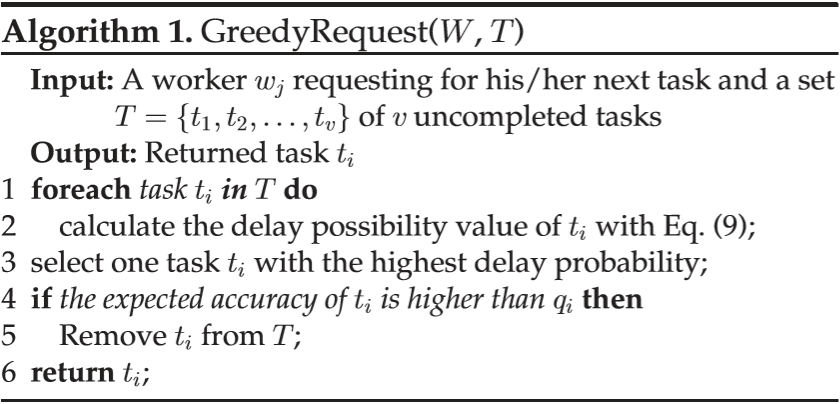
\includegraphics[width= 0.65\linewidth]{ALGO1.png}
     \end{figure}
     Where the delay probability $L(t_i)$ of task $t_i$ is estimated by:
     $$
     L\left(t_{i}\right) \propto\left(d_{i} \cdot q_{i}\right)^{\left\lceil\frac{\epsilon_{\max }-\epsilon_{i}}{r_{l}}\right\rceil}
     $$
     where $d_i$ is the difficulty of task $t_i$ and $\epsilon_i$ 
     is the time lapse of task $t_i$.\footnote[1]{For more information, refer to the original paper.}
\end{frame}

\begin{frame}
    \frametitle{Batch-Based Scheduling (BBS) Approach}
    Strategy: assign high-accuracy workers to 
    difficult and urgent tasks and low-accuracy 
    workers with easy and not that urgent tasks
    \begin{figure}
        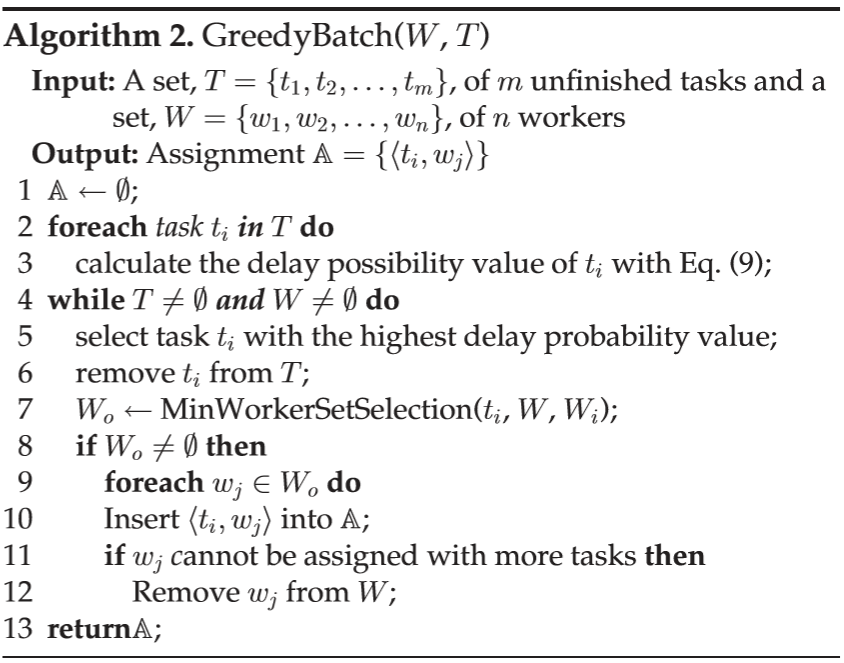
\includegraphics[width= 0.6\linewidth]{ALGO2.png}
     \end{figure}
    \footnote{\texttt{MinWorkerSetSelection} selects a minimum set of workers 
    satisfying the constraint of the 
    quality threshold for task $t_i$}
\end{frame}

\begin{frame}
    \frametitle{Time Complexity}
    \begin{block}{Request-Based Scheduling Approach}
        Assume that each task has received $h$ answers. Then
        with $v$ uncompleted tasks, the time complexity of RBS algorithm is
        $$O(v \cdot h)$$
    \end{block}
    \begin{block}{Batch-Based Scheduling Approach}
        Assume that each task $t_i$ needs to be answered 
        by $h$ workers, then the time complexity of BBS alrogithm is
        $$O(m \cdot h)$$
    \end{block}
\end{frame}

\section{The Notification Module}
\subsection{Definitions}

\begin{frame}
    \frametitle{Worker Dominance}
    Given two worker candidates $w_x$ and $w_y$, 
    we say worker $w_x$ dominates worker $w_y$, 
    if it holds that:
    \begin{enumerate}
        \item $P_{ts}(w_x) > P_{ts}(w_y)$
        \item $\alpha_x > \alpha_y$
        \item $r_x \leq r_y$
    \end{enumerate}
    where $P_{ts}(wj)$ is the probability that worker $w_j$
    is available, and $a_x$ and $r_x$ are the average 
    accuracy and response time of worker $w_x$ on 
    his/her subscribed categories,respectively.
\end{frame}


\begin{frame}
    \frametitle{Estimation for Worker Availability}
    We can estimate $P_{ts}(w_x)$ using the following methods:
    \begin{block}{Kernel Density Estimation}
        \begin{itemize}
            \item estimate the probability that a worker is available
            based on one’s historical records
            \item has \textbf{``cold-start'' problem}
        \end{itemize}
    \end{block}
    \begin{block}{Smooth Kernel Density Estimation}
        \begin{itemize}
            \item for each worker, use historical data of 
            his/her friends to supplement/predict his/her 
            behaviors
            \item avoids ``cold-start'' problem
        \end{itemize}
    \end{block}
\end{frame}

\subsection{Efficient Worker Notifying Problem}
\begin{frame}
    \frametitle{Efficient Worker Notifying Problem}
    Given a timestamp $t_s$, a set $W$ of $n$ offiine 
    workers, the historical online records $E_j = \{e_1, e_2, \cdots , e_n\}$ 
    of each worker $w_j$, and the number, $u$, of 
    workers that we need to recruit for the public 
    worker pool, the problem of efficient worker notifying is
    to \textbf{select a subset of workers in $W$ with 
    high accuracies and low latencies to send 
    invitation messages}, such that:
    \begin{enumerate}
        \item  The expected number, $E(P_{ts}(W))$ 
        of workers who accept the invitations is greater than $u$
        \item The number of workers in $W$, to whom we send notifications, 
        is minimized, where $P_{ts}()$ is the probability of 
        workers to accept invitations and log in the worker 
        pool at timestamp $ts$. 
    \end{enumerate}
\end{frame}

\begin{frame}
    \frametitle{Solving of the EWN Problem }
    \begin{figure}
        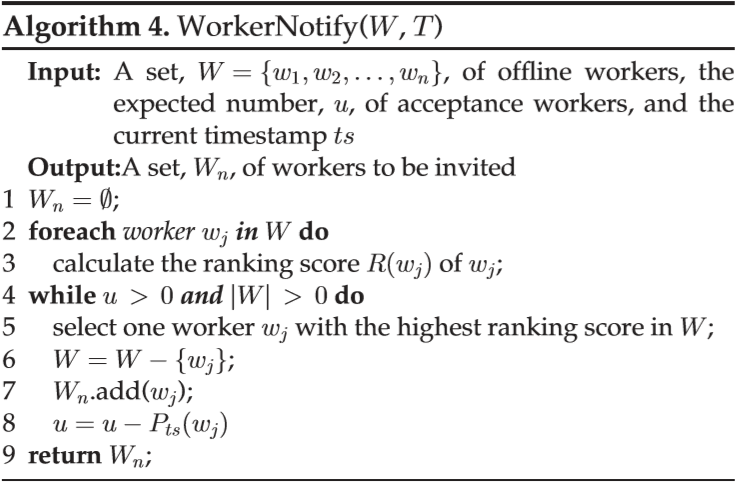
\includegraphics[width= 0.65\linewidth]{ALGO3.png}
     \end{figure}
     Where the ranking score $R(w_j)$ represents the dominance
     of the worker $w_j$.
\end{frame}

\section{Experimental Results}

\begin{frame}
    \frametitle{Performance of Task Scheduler Module}
    \begin{figure}
        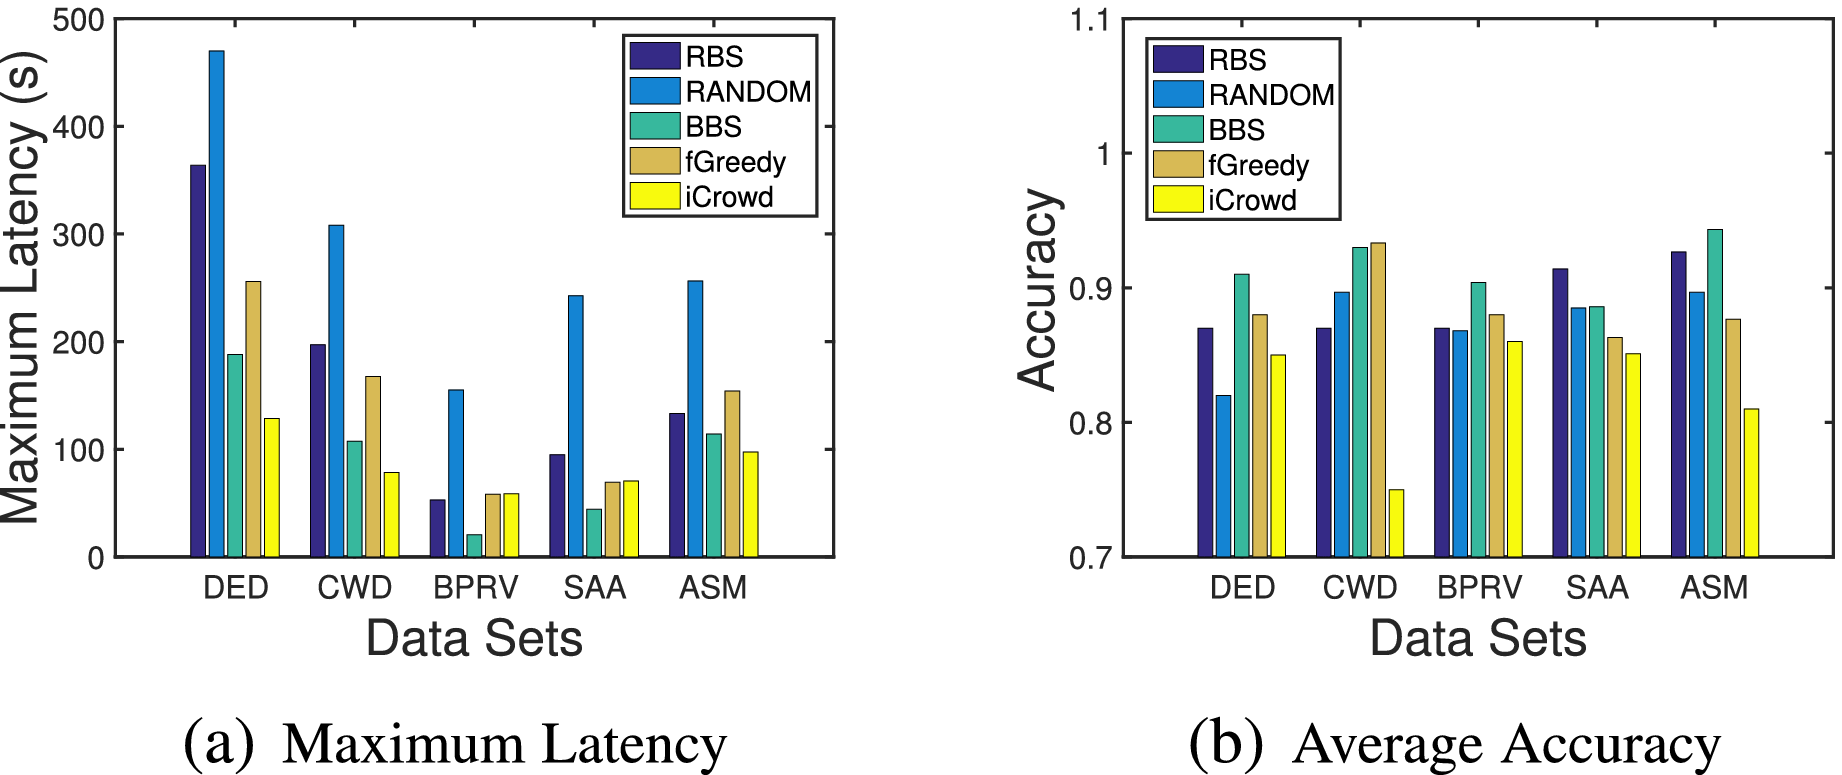
\includegraphics[width= 0.95\linewidth]{chen2-2849394-hires.png}
     \end{figure}
\end{frame}

\begin{frame}
    \frametitle{Performance of the Notification Module}
    \begin{figure}
        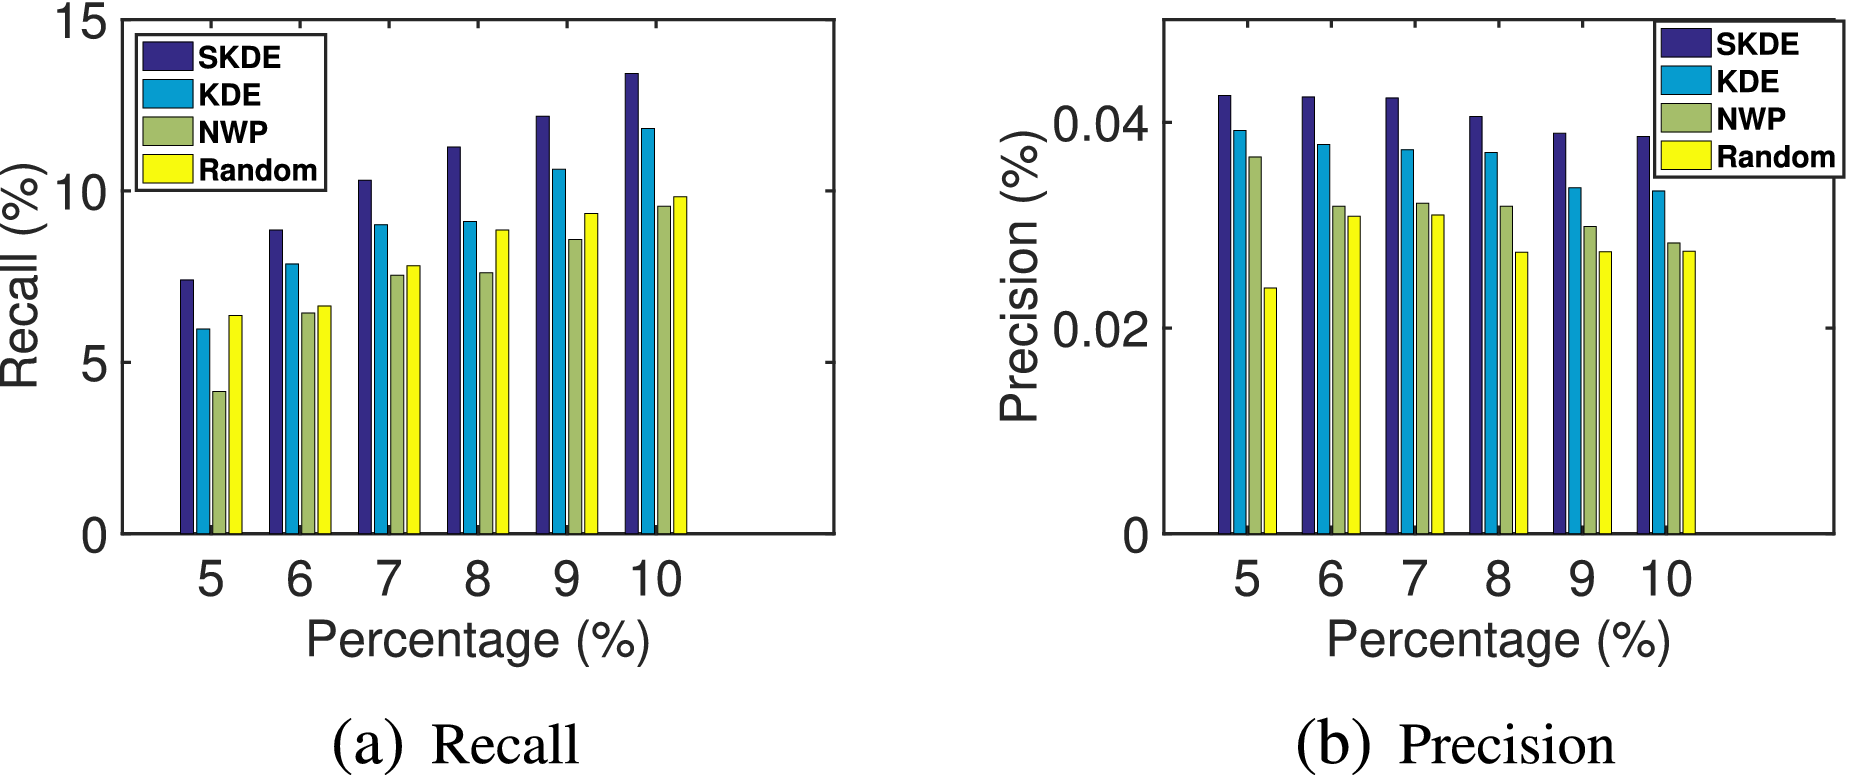
\includegraphics[width= 0.95\linewidth]{chen3-2849394-hires.png}
     \end{figure}
\end{frame}

\begin{frame}
    \frametitle{Effect of the number of tasks $m$}
    \begin{figure}
        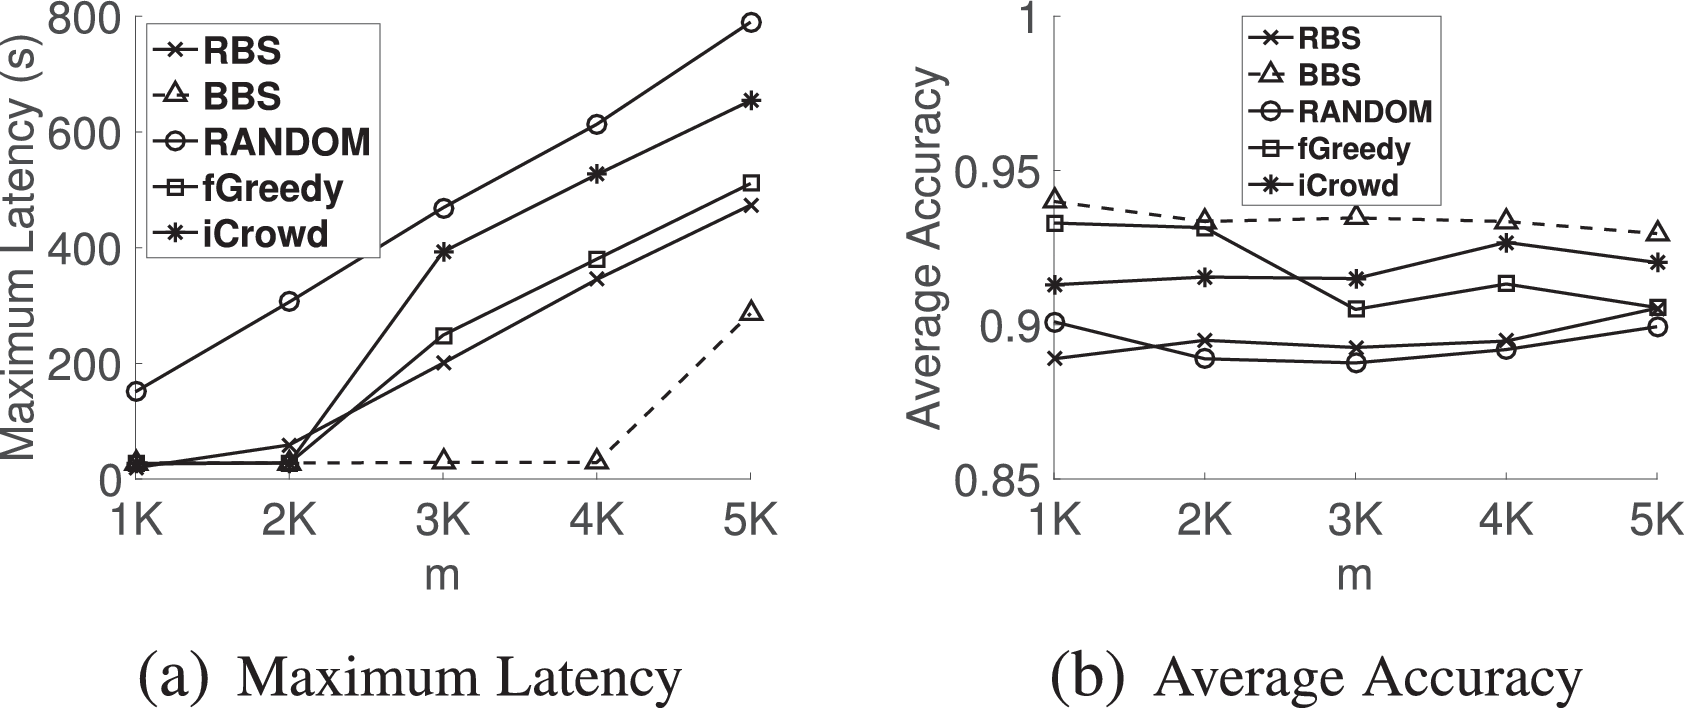
\includegraphics[width= 0.95\linewidth]{chen4-2849394-hires.png}
     \end{figure}
\end{frame}

\begin{frame}
    \frametitle{Effect of the number of workers $n$}
    \begin{figure}
        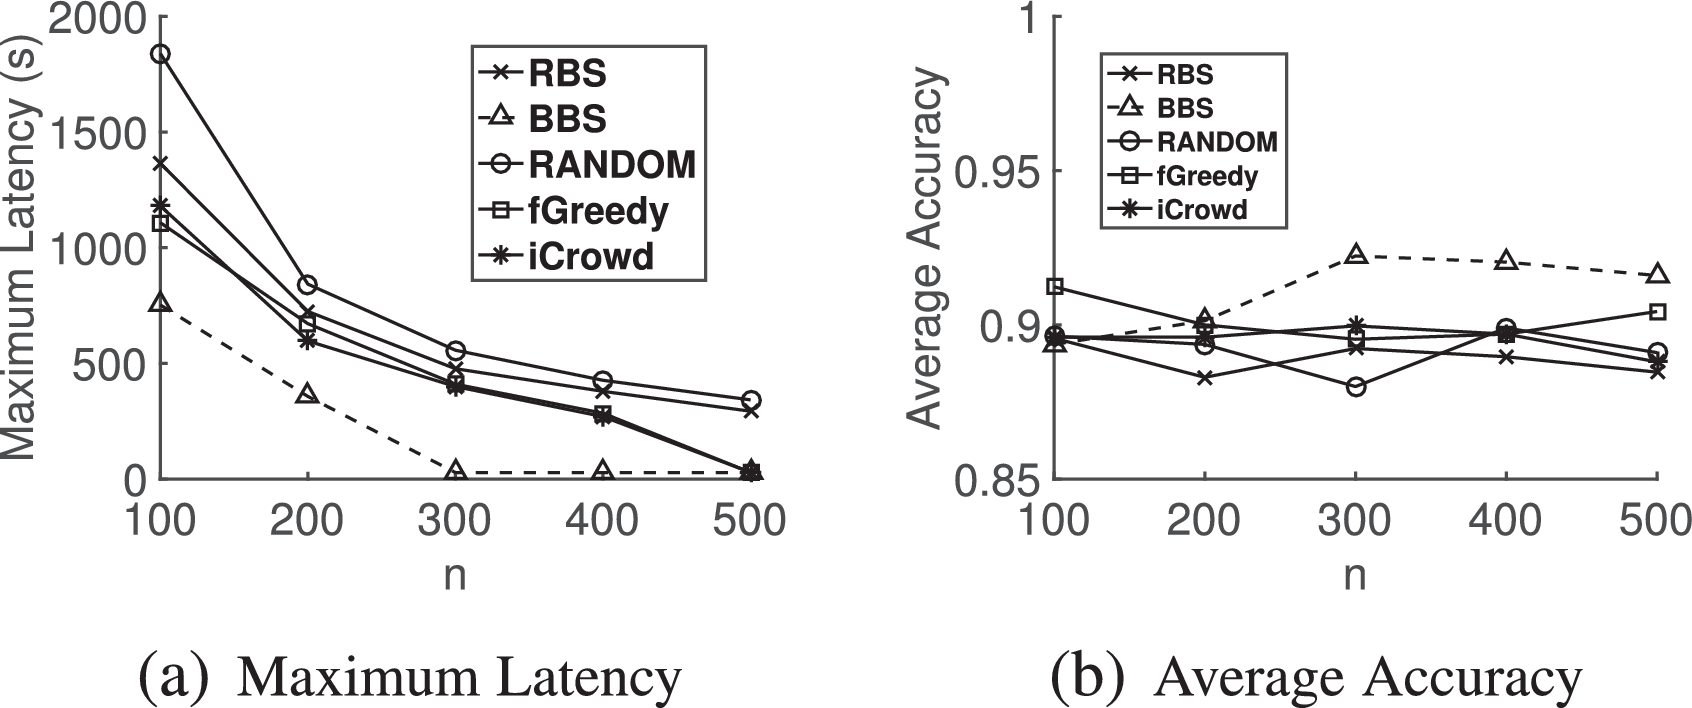
\includegraphics[width= 0.95\linewidth]{chen5-2849394-hires.png}
     \end{figure}
\end{frame}

\begin{frame}
    \frametitle{Effect of the specific quality value range $[q^-, q^+]$}
    \begin{figure}
        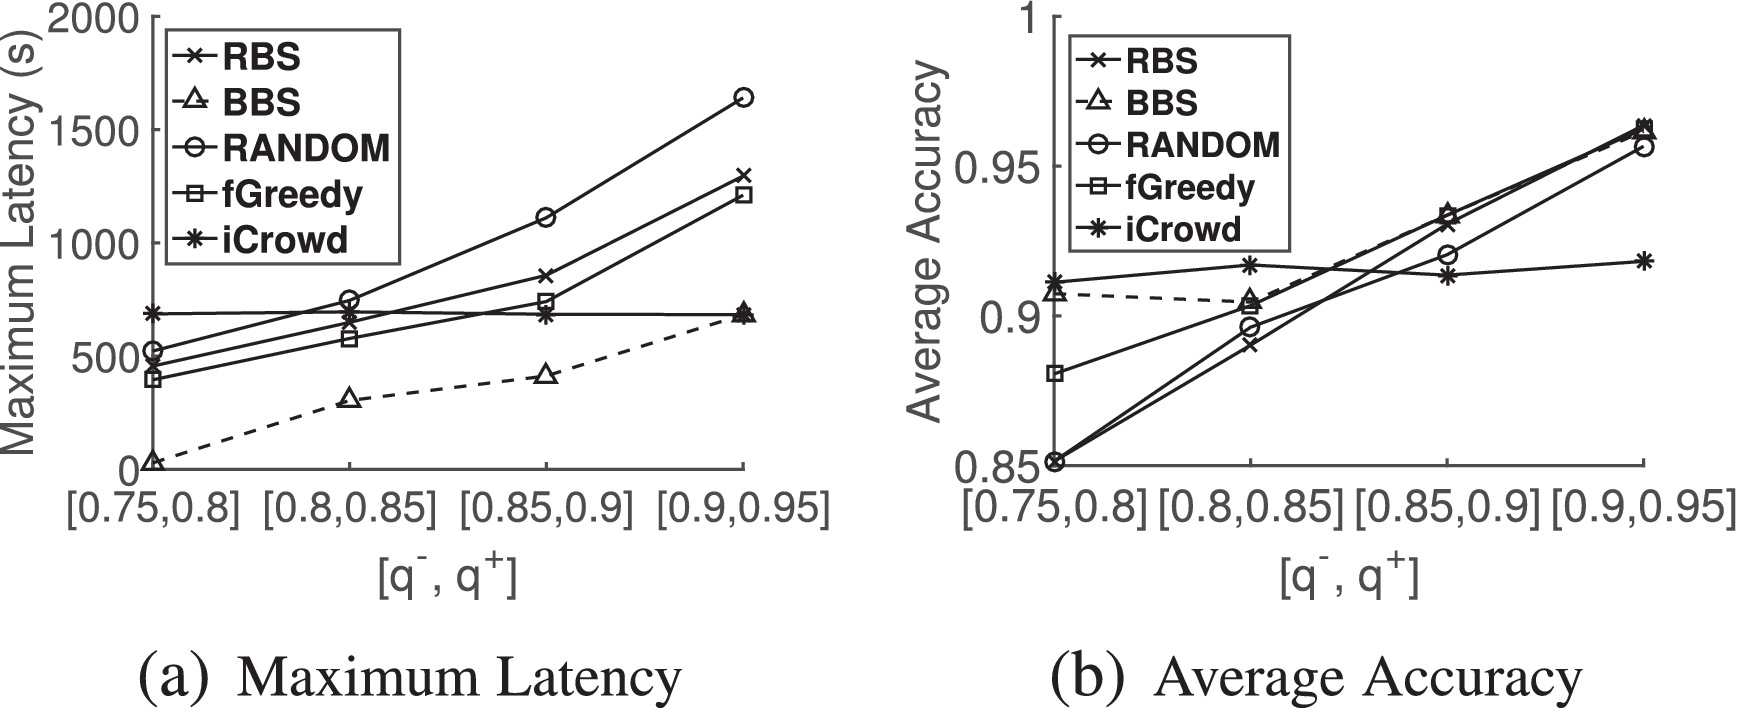
\includegraphics[width= 0.95\linewidth]{chen6-2849394-hires.png}
     \end{figure}
\end{frame}

\begin{frame}
    \frametitle{Effect of the number of categories $l$}
    \begin{figure}
        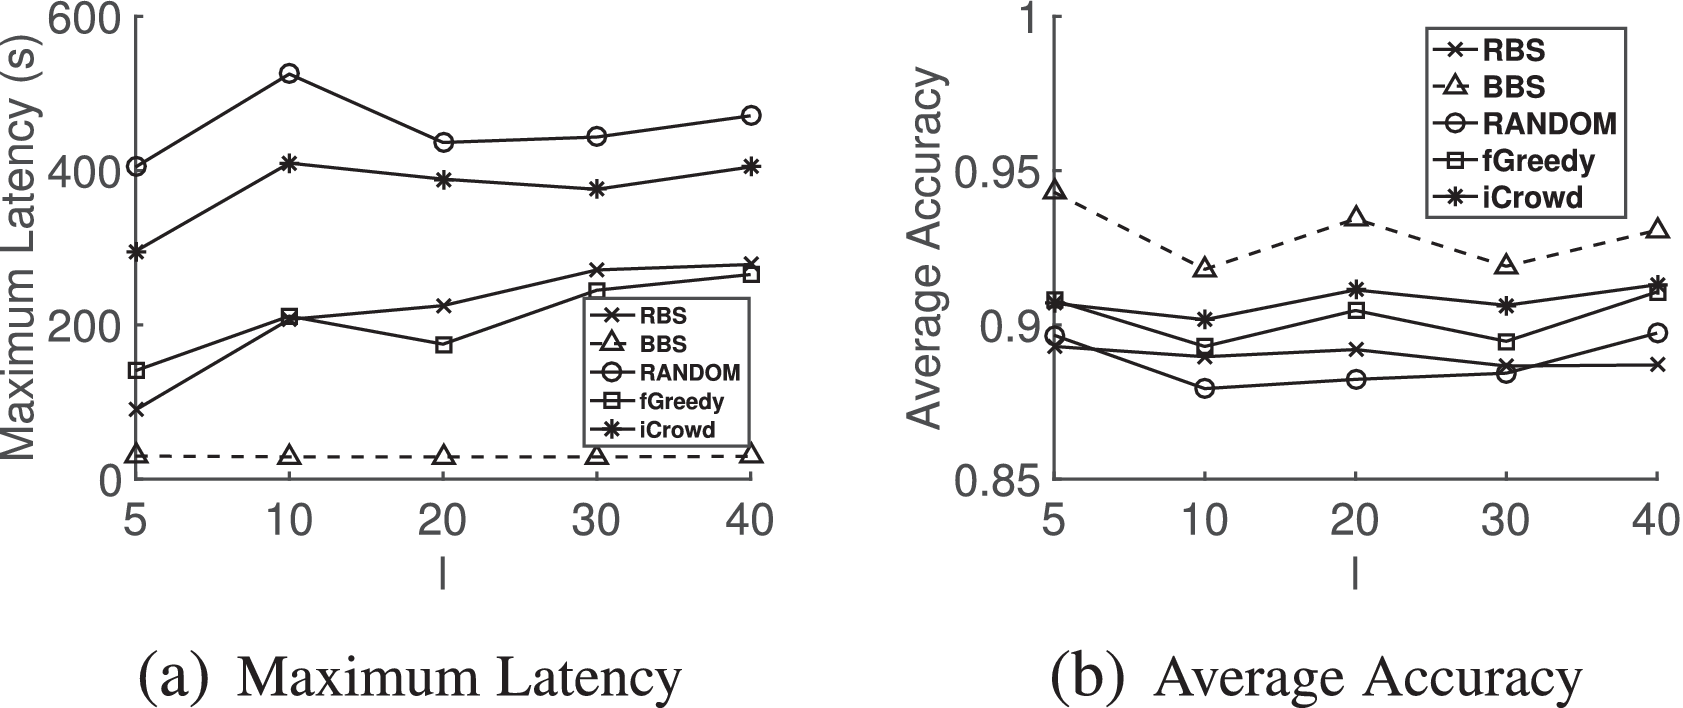
\includegraphics[width= 0.95\linewidth]{chen7-2849394-hires.png}
     \end{figure}
\end{frame}

\section{Conclusion}

\begin{frame}
    \frametitle{Conclusion}
    In this paper, the authors
    \begin{itemize}
        \item  propose a novel fast
        and reliable crowdsourcing(FROG) framework
        \item  formalize the FROG task scheduling(FROG-TS)
        and efficient worker notifying (EWN) problems
        \item proposed effective and efficient approaches
        to solve the problems
        \item demonstrate the effectiveness and efficiency 
        of our proposed FROG framework 
        on both real and synthetic data sets
    \end{itemize}
\end{frame}

\begin{frame}
    \begin{center}
        \Huge Thank You
    \end{center}
\end{frame}

\end{document}